% Paste-ready figure blocks for essay.tex.
% Nothing here is included automatically: copy a block into essay.tex where noted.
% Figures are regenerated with:  python3 latex/figures/make_figures.py
%
% Paths are relative to latex/ (where essay.tex is compiled), so no
% \graphicspath change is needed. Captions sit below the figure in italics,
% matching your existing \captionsetup and sample essay 1.

% ---------------------------------------------------------------------------
% Figure 1 - Big Earth data workflow
% Suggested place: end of "Global Monitoring Baseline", right after the
% paragraph that ends "...support IUU-fishing ... analysis \parencite{unep2024}."
% Suggested sentence before it:
%   Figure~\ref{fig:workflow} summarises how these data streams become SDG 14 indicators.
% ---------------------------------------------------------------------------
\begin{figure}[!htb]
\centering
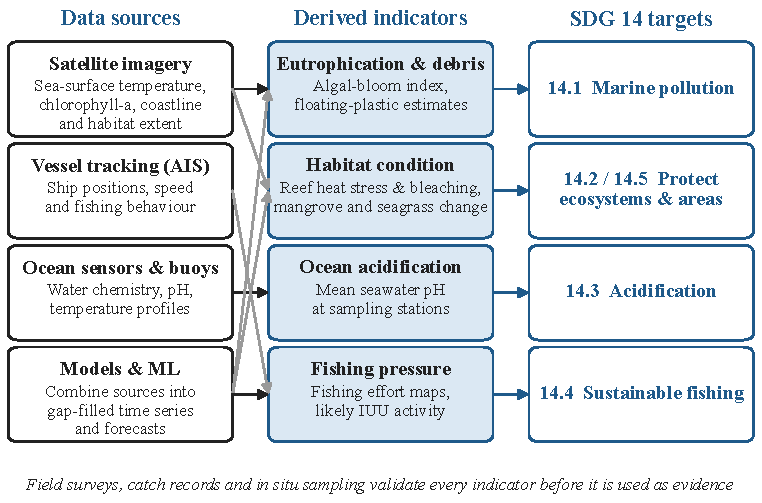
\includegraphics[width=\textwidth]{figures/bigdata_workflow.pdf}
\caption{How Big Earth data sources feed indicators for SDG 14 targets
(author's synthesis based on \cite{unep2024} and \cite{jpl2024}).}
\label{fig:workflow}
\end{figure}

% ---------------------------------------------------------------------------
% Figure 2 - MPA coverage by country
% Suggested place: just before Table~\ref{tab:countries} (end of
% "Japan and India"), so readers see the numbers before the summary table.
% Suggested sentence before it:
%   Figure~\ref{fig:mpa} compares reported protected-area coverage against the
%   10-percent and 30-percent targets; China, Japan and India publish no
%   directly comparable percentage.
% ---------------------------------------------------------------------------
\begin{figure}[!htb]
\centering
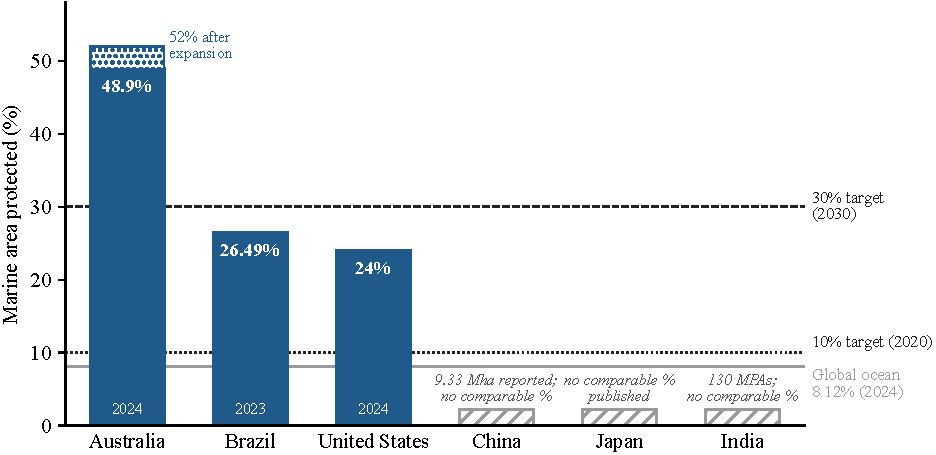
\includegraphics[width=\textwidth]{figures/mpa_coverage.pdf}
\caption{Reported marine protected-area coverage of national waters compared
with the 2020 and 2030 targets. Hatched bars mark countries without a
comparable published percentage. National figures as cited in the country
sections; global coverage from \cite{un2024}.}
\label{fig:mpa}
\end{figure}
